\maketitle
\tableofcontents
\newpage

\section{Zielsetzung}
In diesem Versuch geht es um Messung der Schwingungs- und Schwebungsdauer von gekoppelten Pendeln.
Untersucht werden gleich- und gegensinnige sowie gekoppelte Schwingungen.
\section{Theorie}
Ein einzelndes Fadenpendel, welches reibungsfrei aufgehängt wurde, mit einem Faden der Länge $\textit{l}$ und Masse $\textit{m}$
schwingt für kleine Auslenkungen (sin $\phi \approx \phi$) mit der Schwingungsfrequenz
\begin{equation}
  \omega = \sqrt{\frac{\textit{l}}{g}}
  \label{e1}
\end{equation}
Dies ist die Lösung der zugehörigen Schwingungsdifferentialgleichung mit g als Erdbeschleunigungskonstante. Mit \eqref{e1} und
\begin{equation*}
  \textit{T} = \frac{2\pi}{\omega}
\end{equation*}
ergibt sich als Formel für die gesuchte Schwingungsdauer
\begin{equation}
  \textit{T} = 2\pi \sqrt{\frac{g}{\textit{l}}}
  \label{e2}
\end{equation}
Wenn man nun zwei dieser Fadenpendel durch eine Feder koppelt, ergeben sich zwei DGL's mit jeweils einem Term darin,
der den Drehwinkel des anderen Pendels enthält. Dies kommt durch die Kopplung mit der Feder. Je nach Auslenkungswinkel $\alpha_{1}$
und $\alpha_{2}$ der Fadenpendel ergeben sich verschiedene Schwingungsarten:
\\
\\
Für: $\alpha_{1} = \alpha_{2}$ ergibt sich eine gleichsinnige Schwingung. Bei dieser hat die Feder keine Auswirkung auf die
Schwingungen. Deshalb gilt für die Schwingungsfrequenz $\omega_{+}$ \eqref{e1} und für die Schwingungsdauer $\textit{T}_{+}$
\eqref{e2}.
\\
\\
Wenn $\alpha_{1} = -\alpha_{2}$ ist, nennt man dies eine gegensinnige Schwingung. Für diesen Fall greift die Feder in das Schwingverhalten
der Pendel ein. Deshalb werden \eqref{e1} und \eqref{e2} erweitert um jeweils einen Term mit der Kopplungskonstante $\textit{K}$
der Feder
\begin{equation}
  \omega_{-} = \sqrt{\frac{l}{g} + \frac{2 \textit{K}}{l}}
  \label{e3}
\end{equation}
\begin{equation}
  \textit{T}_{-} = 2\pi  \sqrt{\frac{l}{g + 2 \textit{K}}}
  \label{e4}
\end{equation}
\\
\\
Für: $\alpha_{1} = 0, \alpha_{2} \neq 0$ ergibt sich eine gekoppelte Schwingung. Diese zeichnet sich dadurch aus, dass die beiden
Pendel die kinetische Energie auf das andere Pendel übertragen und dann erneut erhalten. Hier tritt die sogenannte Schwebung auf.
Dieser Begriff beschreibt die Zeit zwischen zwei Stillständen eines Pendels. Die Dauer dieses Zustandes berechnet sich nach
\begin{equation}
  \textit{T}_{S} = \frac{\textit{T}_{-} \cdot \textit{T}_{+}}{\textit{T}_{+} - \textit{T}_{-}}
  \label{e5}
\end{equation}
mit $\textit{T}_{-}$ aus der gegen- und $\textit{T}_{+}$ aus der gleichsinnigen Schwingung. Die Kopplungskonstante \textit{K}
der Feder zwischen den beiden Pendeln definiert sich nach
\begin{equation}
  \textit{K} = \frac{\textit{T}_{+}^{2} - \textit{T}_{-}^{2}}{\textit{T}_{+}^{2} + \textit{T}_{-}^{2}}
  \label{e6}
\end{equation}
\section{Durchführung}
Die Pendel sind zwei Stabpendel, die verschiebbare Massen besitzen, um verschiedene Pendellängen zu realisieren. Die
Aufhängung besteht aus einer reibungsarmen Spitzenlagerung, die eine reibungsfreie Schwingung gewährleistet.
\begin{figure}
  \centering
  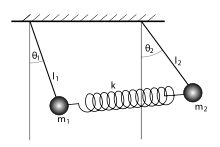
\includegraphics{gekoppelte_pendel.png}
  \caption{Darstellung eines gekoppelten Pendels mit Öffnungswinkel $\theta$ statt $\alpha$.}
  \label{fig:skizze1}
\end{figure}
Alle Schwingungsdauern werden für fünf Schwingungen und für eine Pendellänge von 0,6 $\textit{m}$ bestimmt. Zuerst messen wir die Schwingungsdauern $\textit{T}_{1}$
und $\textit{T}_{2}$ der einzelnen Pendel nach und vergleichen, ob sie im Rahmen der Messgenauigkeit übereinstimmen. Um eventuellen
statistischen Fehlern vorzubeugen, führen wir die Messung neunmal aus. Danach verbinden wir die beiden Pendel über die Kopplungsfeder und führen eine gleich-
und eine gegensinnige Schwingung durch , wobei wir $\textit{T}_{+}$ und $\textit{T}_{-}$ experimentell bestimmen. Im
Anschluss ermitteln wir die Schwebungsdauer $\textit{T}_{S}$ und die Schwingungsdauer $\textit{T}$. Zum Schluss wiederholen wir
alle Messungen für eine Pendellänge von 0,75 $\textit{m}$.
\section{Auswertung}
\section{Diskussion}
\newpage
\nocite{*}
\printbibliography
